% ******************************************************** %
%              TEMPLATE DE INFORME ORGA2 v0.1              %
% ******************************************************** %
% ******************************************************** %
%                                                          %
% ALGUNOS PAQUETES REQUERIDOS (EN UBUNTU):                 %
% ========================================
%                                                          %
% texlive-latex-base                                       %
% texlive-latex-recommended                                %
% texlive-fonts-recommended                                %
% texlive-latex-extra?                                     %
% texlive-lang-spanish (en ubuntu 13.10)                   %
% ******************************************************** %
\documentclass[a4paper]{article}
\usepackage[spanish]{babel}
\usepackage[utf8]{inputenc}
\usepackage{charter}   % tipografia
\usepackage{graphicx}
%\usepackage{makeidx}
\usepackage{paralist} %itemize inline
\usepackage{algorithm}  % implementacion ondas en C
% sudo apt-get install texlive-science
\usepackage{algorithmic} % implementacion ondas en C
%\usepackage{float}
\usepackage{amsmath, amsthm, amssymb}
%\usepackage{amsfonts}
%\usepackage{sectsty}
%\usepackage{charter}
%\usepackage{wrapfig}
%\usepackage{listings}
%\lstset{language=C}
% \setcounter{secnumdepth}{2}
\usepackage{wrapfig}
\usepackage{underscore}
\usepackage{caratula}
\usepackage{url}
\usepackage{multicol}
\usepackage{algpseudocode}

% ********************************************************* %
% ~~~~~~~~              Code snippets             ~~~~~~~~~ %
% ********************************************************* %
\usepackage{color} % para snipets de codigo coloreados
\usepackage{fancybox}  % para el sbox de los snipets de codigo
\definecolor{litegrey}{gray}{0.94}
\newenvironment{codesnippet}{%
	\begin{Sbox}\begin{minipage}{\textwidth}\sffamily\small}%
	{\end{minipage}\end{Sbox}%
		\begin{center}%
		\vspace{0cm}\colorbox{litegrey}{\TheSbox}\end{center}\vspace{0cm}}
% ********************************************************* %
% ~~~~~~~~         Formato de las páginas         ~~~~~~~~~ %
% ********************************************************* %
\usepackage{fancyhdr}
\pagestyle{fancy}
%\renewcommand{\chaptermark}[1]{\markboth{#1}{}}
\renewcommand{\sectionmark}[1]{\markright{\thesection\ - #1}}
\fancyhf{}
\fancyhead[LO]{Sección \rightmark} % \thesection\ 
\fancyfoot[LO]{\small{Centeno, Romera, Ghianni}}
\fancyfoot[RO]{\thepage}
\renewcommand{\headrulewidth}{0.5pt}
\renewcommand{\footrulewidth}{0.5pt}
\setlength{\hoffset}{-0.8in}
\setlength{\textwidth}{16cm}
%\setlength{\hoffset}{-1.1cm}
%\setlength{\textwidth}{16cm}
\setlength{\headsep}{0.5cm}
\setlength{\textheight}{25cm}
\setlength{\voffset}{-0.7in}
\setlength{\headwidth}{\textwidth}
\setlength{\headheight}{13.1pt}
\renewcommand{\baselinestretch}{1.1}  % line spacing
% ******************************************************** %

\begin{document}

\thispagestyle{empty}
\materia{Sistemas Operativos}
\submateria{Segundo Cuatrimestre de 2019}
\titulo{Trabajo Práctico I}
\integrante{Joaquin P. Centeno}{699/16}{joaquinpcenteno@gmail.com}
\integrante{Joaquin Romera }{183/16}{joakromera@gmail.com}
\integrante{Hernán Ghianni}{538/16}{herghia@gmail.com}

\maketitle

\newpage

\thispagestyle{empty}
\vfill
\thispagestyle{empty}
\vspace{3cm}

\tableofcontents
\newpage

\section{Introducción}

En este trabajo se propone una solución para resolver el problema de encontrar árboles generadores mínimos de grafos (AGM) con múltiples threads, evitando deadlocks y otros problemas asociados. El algoritmo tradicional es Prim ejecutado como un único thread en un proceso, empezando en un nodo y avanzando siempre por el eje de menor peso hacia el próximo vecino no visitado.

Nuestra propuesta permite elegir la cantidad de threads que van a encontrar un AGM para un grafo determinado, al momento de ejecución se utiliza una versión paralela del antes mencionado algoritmo de Prim, replicado en tantos hilos como hayan sido elegidos el mismo algoritmo pero iniciando cada uno desde un nodo diferente del mismo grafo.

Los problemas potenciales que pueden existir en esta estrategia surgen cuando más de un thread quiere capturar el mismo nodo, o cuando uno o más threads quiere capturar un nodo perteneciente a otro thread. A estos escenarios se suma la complejidad de resolver ciclos cuando dos threads se quieren fusionar mutuamente, y aquellos relacionados con la naturaleza de la programación asincrónica y paralela: evitar deadlocks, starvations, race conditions y asegurar la contención. Un esquema simple para resolver estas dificultades fue propuesto utilizando locks y trylocks de la libreria Pthreads.

Se presentan resultados de experimentaciones para analiza el método propuesto.

\subsection{AGM}

El problema del Árbol Generador Mínimo fue resuelto por primera vez en 1926 día de hoy tiene numerosas aplicaciones en organización, ruteo y partición de redes. La definición del problema es la siguiente: dado un grafo conexo y no dirigido G con pesos en sus ejes, encontrar el árbol generador de peso total mínimo. Es decir, encontrar un subgrafo que sea un árbol, que contenga a todos los vértices de G y tal que la suma de los pesos de los ejes del subgrafo sea igual o menor a la de cualquier otro árbol generador de G.

Para resolver este problema utilizamos una variante del algoritmo de Prim. La misma es parametrizable en la cantidad de threads, permitiendo la búsqueda del AGM desde distintos nodos del grafo en diferentes hilos de ejecución.

\subsection{Programación paralela y Pthreads}

Un proceso es un programa en ejecución. El objetivo de utilizar paralelismo es optimizar la resolución de un problema, partiéndolo en unidades más pequeñas que puedan ejecutarse en paralelo. Para esto utilizamos threads (con la librería pthreads), una alternativa más eficiente a múltiples procesos (por medio de forks).

Al utilizar threads se comparte el mismo espacio de direcciones, lo cual facilita compartir datos entre diferentes hilos. De esta manera, la estructura del grafo y sus 'colores' son compartidos, cada thread crece su propio agm, pintando cada nodo del mismo con su ID. Es necesario garantizar la contención en los casos que distintos hilos quieran acceder a las mismas estructuras en el mismo momento. Para esto hacen falta ciertas estructuras para la sincronización que serán explicadas en las siguientes secciones del informe.
\newpage
\section{Desarrollo}

En esta sección damos un detalle de las estructuras que utilizamos para mantener la contención y sincronización entre los diferentes hilos del proceso. Luego, explicamos a alto nivel el pseudocódigo correspondiente a nuestro algoritmo.

\subsection{Estructuras}

\begin{figure}[h]
    \centering
    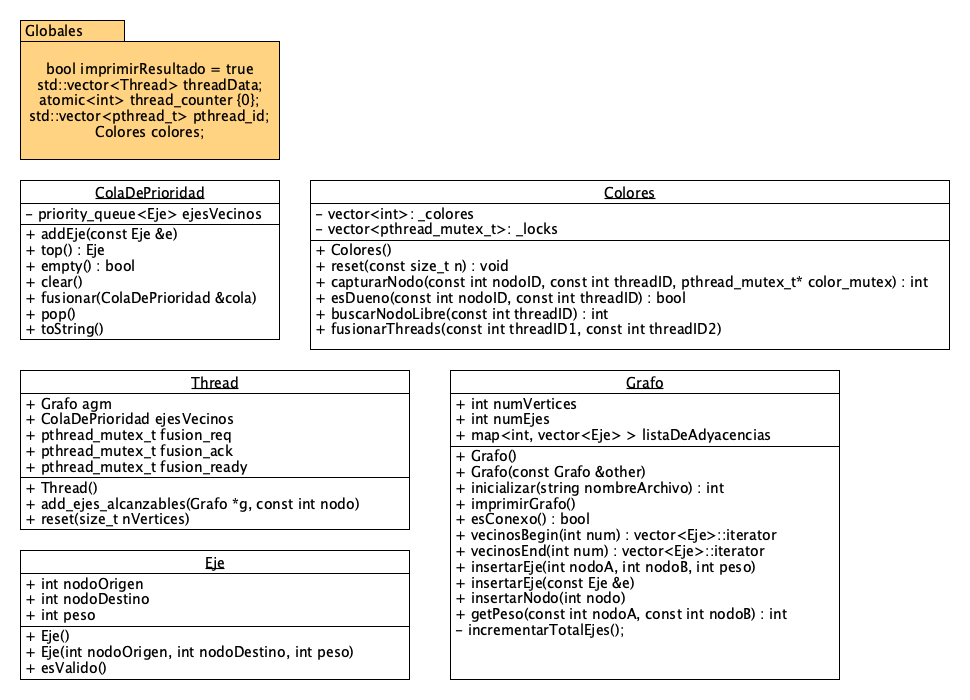
\includegraphics[width=1\textwidth]{imagenes/tp1.png} \\%
    \caption{Clases y estructuras}
    \label{fig:uml}
\end{figure}

\subsubsection{Variables globales}

En la memoria compartida por cada proceso se encuentra la información correspondiente a cada thread en \textbf{threadData}, el \textit{ownership} de cada nodo en \textbf{colores}, un contador atómico para identificar los threads durante su inicialización, \textbf{thread_counter} y finalmente un vector de \textit{pthread_t} para coordinar la creación de los threads y para esperar a que los mismos terminen: \textbf{pthread_id}.

Estos objetos se encuentran en: \textmd{/src/globales.h}

\subsubsection{Grafos y Ejes}

Se utilizaron las estructuras facilitadas por la cátedra con leves modificaciones. En el caso de los grafos se agregó un constructor por copia y se sobrecargó el método de \textbf{insertarEje}, también incluyeron: \textbf{insertarNodo} y \textbf{getPeso} para facilitar algunas operaciones.

En el caso de los ejes, se agregó información correspondiente al nodo de origen y un constructor con distintos parámetros.

Ver \textmd{/src/grafo.h}

\newpage

\subsubsection{Thread}

\begin{verbatim}
    struct Thread{
        Grafo agm;
        ColaDePrioridad ejesVecinos;
        pthread_mutex_t fusion_req;
        pthread_mutex_t fusion_ack;
        pthread_mutex_t fusion_ready;
    };
\end{verbatim}

Trabajamos con esta estructura para resguardar la información de cada thread. La misma consiste de un grafo que será el AGM parcial del thread, una cola de prioridad que contiene a los ejes cuyo nodo destino es alcanzable desde el AGM y tres mutex para administrar las fusiones. Tendremos un vector global que contendrá uno de estos structs por cada thread, el nombre del mismo es threadData.

Ver \textmd{/src/thread.h}

\subsubsection{Cola De Prioridad}

Cada thread tiene una cola de prioridad, \textbf{ejesVecinos}, que mantiene ordenados crecientemente los ejes actualmente alcanzables según su peso. A la hora de buscar el próximo nodo a capturar, siempre se eligirá el primer elemento de la cola. Luego de capturar un nodo, sus ejes son agregados a la misma y el proceso se repite.

Ver \textmd{/src/cola_proridad.h}

\subsubsection{Colores}

\begin{verbatim}
    class Colores {
        vector<int> _colores;
        vector<pthread_mutex_t> _locks;
    };
\end{verbatim}

Para controlar que la pertenencia de los nodos del grafo utilizamos esta estructura que contiene un vector con el color de cada uno, los cuales no son otra cosa que los ID de cada thread. Para evitar race conditions y asegurar contención, cada nodo tiene además un mutex asociado el cual nos permite tener acceso exclusivo al mismo. Vamos a distinguir además a los nodos libres con un -1.  Las operaciones principales de la clase son \textbf{esDueño} que nos permite conocer al thread que posee a ese nodo y \textbf{capturarNodo} cuyo objetivo es convertir a un thread en dueño de un nodo. En caso de que esto ultimo no sea posible, porque ya pertenece a otro thread, se procederá a solicitar una fusión. Cuando esta se produzca los nodos del thread de mayor id cambiaran de dueño y pasaran a ser del de menor id.

Ver \textmd{/src/colores.h}

\subsubsection{Fusión}

Como mencionamos anteriormente, cada thread cuenta con tres mutex para administrar tanto la solicitud como la habilitación de fusiones. En cada ciclo los threads van a chequear si tienen fusiones entrantes haciendo trylock de su mutex fusion\_req. Mientras no puedan tomarlo implica que otro thread está esperando para fusionarse. Si lo pueden tomar, se hace un unlock de su fusion\_ack despertando al thread solicitante y un lock de fusion\_ready, este último es para esperar a que el otro thread solicitante termine de realizar la fusión.

Una vez que ya no tiene pendientes procede a buscar el próximo nodo e intentar capturarlo. En caso de que pertenezca a otro thread solicita una fusión de la siguiente forma: primero chequea que no tenga funciones entrantes haciendo un trylock de su fusion\_req. Esto lo hacemos para evitar un posible deadlock. Luego, lo mismo pero con el fusion\_req del thread dueño del nodo que quiere capturar. Si puede conseguirlo hace lock del fusion\_ack del otro thread quedando así en espera hasta que el mismo esté preparado para realizar la fusión. Una vez que la misma se produce se verifica que el dueño siga siendo el mismo ya que podría haber ocurrido una fusión y por lo tanto haber cambiado. Si se mantuvo se debe chequear cuál es el de menor id, el cual será quien "sobreviva". El otro será reiniciado y comenzará de nuevo con todo el proceso. El sobreviviente tendrá ahora la unión de ambos AGMs y ambas colas de prioridad.

Por ultimo, ambos fusion\_req serán desbloqueados, así como el fusion\_ready del perdedor. Es importante remarcar que el thread reiniciado mantiene el estado de sus mutex ya que, si no, podría ocurrir que algún thread quede esperando fusionarse con él. Si no hubiera sido posible conseguir alguno de los fusion\_req o el dueño del nodo hubiera cambiado el thread habría vuelto al principio de este ciclo.

Ver \textmd{/src/fusiones.h} y \textbf{mstParaleloThread} en \textmd{/src/tp1_grafo.cpp}

\subsection{Algoritmo}

\begin{algorithm}
\caption{mstParaleloThread}
\begin{algorithmic}

\STATE $my\_id \gets thread\_counter++ $
\STATE $eje\_actual$
\STATE $my\_data \gets threadData[my\_id]$
\WHILE{$true$}
\STATE $thread\_attend\_fusion\_requests(my\_id)$
\STATE $my\_data.fusion\_req.unlock()$
\STATE $status \gets buscarNodo(my\_id,ejeActual)$
\IF{($status = noHayNodosDisponibles$)}
\STATE $thread\_attend\_fusion\_requests(my\_id)$
\ENDIF
\IF{($status = agmCompleto$)}
\STATE $break$
\ENDIF
\STATE $owner\_id \gets colores.capturarNodo(ejeActual.nodoDestino,my$\textunderscore$id)$
\IF{($my\_id = owner\_id$)}
\STATE $my\_data.insertarEje(ejeActual)$
\STATE $my\_data.agregarEjesVecinos(g,ejeActual.nodoDestino)$
\ELSE 
\STATE $owner\_data \gets threadData[owner\_id]$
\IF{($my\_data.fusion\_req.trylock() \neq 0 )$}
\STATE $continue$
\ENDIF
\IF{($owner\_data.fusion\_req.trylock() \neq 0$)}
\STATE $my\_data.fusion\_req.unlock()$
\STATE $continue$
\ENDIF
\STATE $owner\_data.fusion\_ack.lock()$
\IF{($colores.esDueno(ejeActual,owner\_id)$)}
\STATE $my\_data.agm.insertarEje(ejeActual)$
\IF{($my\_id < owner\_id $)}
\STATE $fuse(my\_id,owner\_id)$
\ELSE
\STATE $fuse(owner\_id,my\_id)$
\ENDIF
\ENDIF
\ENDIF
\STATE $owner\_id.fusion\_req.unlock()$
\STATE $my\_id.fusion\_req.unlock()$
\STATE $owner\_id.fusion\_ready.unlock()$
\ENDWHILE

\end{algorithmic}
\end{algorithm}
\newpage

Aclaraciones:
\begin{itemize}
    \item No realizamos copias del threadData en la implementación. Esto es solamente para clarificar el pseudocódigo.
    \item $thread\_attend\_fusion\_requests$ realiza el chequeo de las funciones entrantes como se explica en la sección 2.1.3.
    \item La idea de buscarNodo es que encuentre el próximo nodo a agregar al agm del thread. Si aun no tiene ninguno toma el primero libre que encuentre. Sino al nodo alcanzable cuyo eje es de peso mínimo. Además de devolver un status retorna el eje en ejeActual.
\end{itemize}

\newpage
\input{2-impl}
\newpage
\section{Experimentación}
\subsection{Mediciones y metodología de experimentación}

Para las mediciones de tiempo se tomó como base la experimentación propuesta
por la cátedra.
% Instancias:
Fueron realizadas mediciones de tiempo para la función \texttt{mstParalelo}
tomando distintas instancias de árboles, grafos ralos y completos, variando la
cantidad de nodos y cantidad de \textit{threads}.
% Repeticiones:
% se repitió 5 veces el llamado a `-e`. Dicho procedimiento usa un for
% i=0,...,9 para correrlo 10 veces obteniendo un total de 50 corridas. El
% procedimiento para correr la experimentación da 1800 filas, nuestro CSV tiene
% 9000 filas.
Debido a la naturaleza no-deterministica de la programación concurrente, se
tomaron 50 corridas para cada instancia (tipo de grafo, cantidad de nodos y
cantidad de \textit{threads}) del problema. En las
figuras~\ref{fig:arboles},~\ref{fig:ralos} y~\ref{fig:completos} se traza el
promedio y se muestra en sombreado el desvío estándar.

% CPU:
Los experimentos fueron medidos en un procesador \texttt{Intel (R) Core (TM) i5
3230M CPU @ 2.60GHz} de 2 \textit{cores} físicos y 4 \textit{cores} lógicos,
con 3072 KB de cache. En una computadora con 8 GB de memoria principal.

\subsection{Resultados}

Se pudo observar que para todos los casos el tiempo de ejecución crece con el
tamaño de la instancia, tanto si su incremento es en cantidad de nodos o en
cantidad de ejes.
% Performance variando #threads
Para todas las instancias obtuvimos una mejor
\textit{performance} al ejecutar de forma secuencial, que al ejecutar más de un
\textit{thread} de forma
concurrente.
% Mas de 4 concurrente:
Puede verse que la degradación de la \textit{performance} se acentúa para las
mediciones de 8, 16 y 32 \textit{threads}, cantidad que supera la cantidad de
\textit{cores} lógicos del CPU donde fueron realizadas las mediciones.

\begin{figure}[h]
\caption{Mediciones para árboles.}
\centering
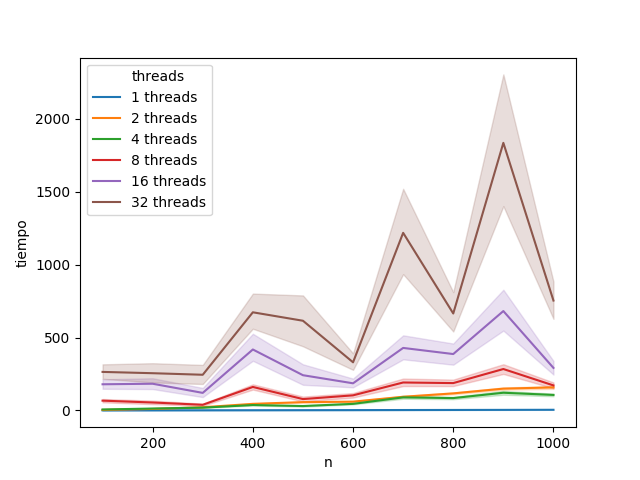
\includegraphics[width=0.5\textwidth]{imagenes/arbol.png} \\%
\label{fig:arboles}
\end{figure}

\begin{figure}[h]
\caption{Mediciones para grafos ralos.}
\centering
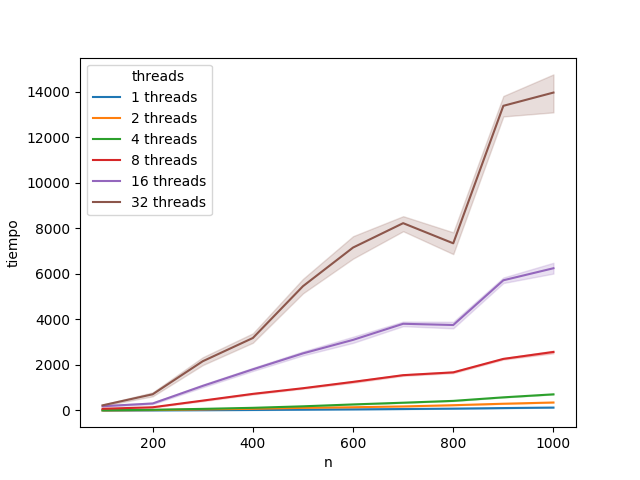
\includegraphics[width=0.5\textwidth]{imagenes/ralo.png} \\%
\label{fig:ralos}
\end{figure}

\begin{figure}[h]
\caption{Mediciones para grafos completos.}
\centering
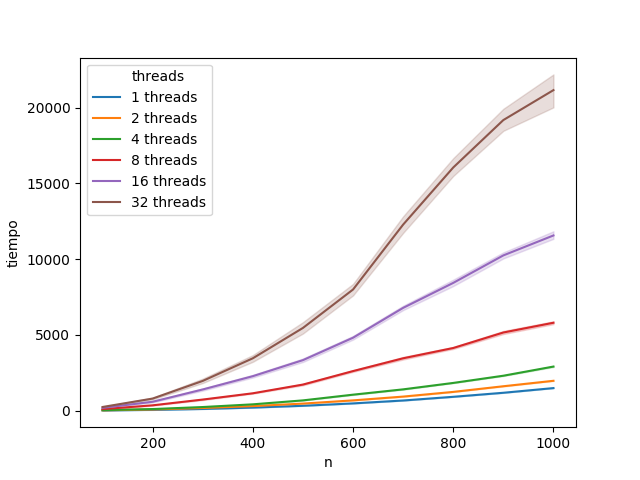
\includegraphics[width=0.5\textwidth]{imagenes/completo.png} \\%
\label{fig:completos}
\end{figure}

%%%%

% Acá hablo de los casos para 1,2,4 threads:
En las figuras~\ref{fig:arboles124}--\ref{fig:completos124} se muestra en
detalle el comportamiento de nuestra implementación del algoritmo para 1, 2 y 4
\textit{threads}. Puede verse que el algoritmo tiene mejor rendimiento de forma
secuencial. Sin embargo para el caso de los árboles, utilizar 4 threads arrojó
mejores resultados que 2, aunque esta diferencia no es significativa.

\begin{figure}[h]
\caption{Mediciones para árboles con hasta 4 \textit{threads}.}
\centering
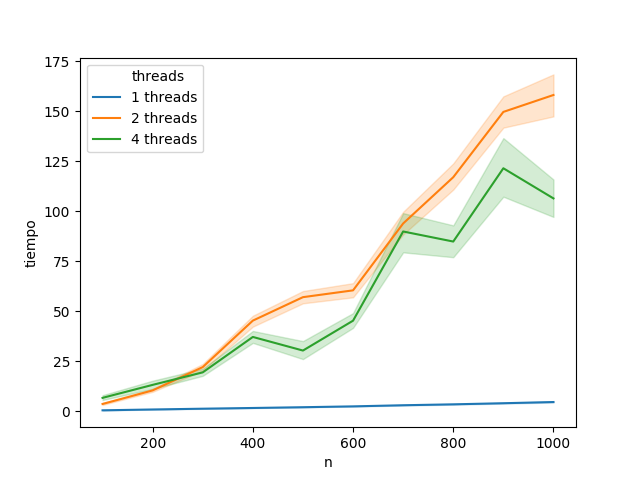
\includegraphics[width=0.5\textwidth]{imagenes/arbol-124.png} \\%
\label{fig:arboles124}
\end{figure}

\begin{figure}[h]
\caption{Mediciones para grafos ralos con hasta 4 \textit{threads}.}
\centering
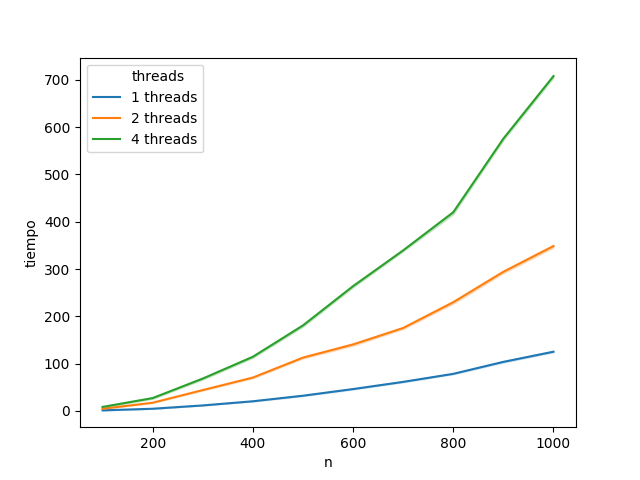
\includegraphics[width=0.5\textwidth]{imagenes/ralo-124.png} \\%
\label{fig:ralos124}
\end{figure}

\begin{figure}[h]
\caption{Mediciones para grafos completos con hasta 4 \textit{threads}.}
\centering
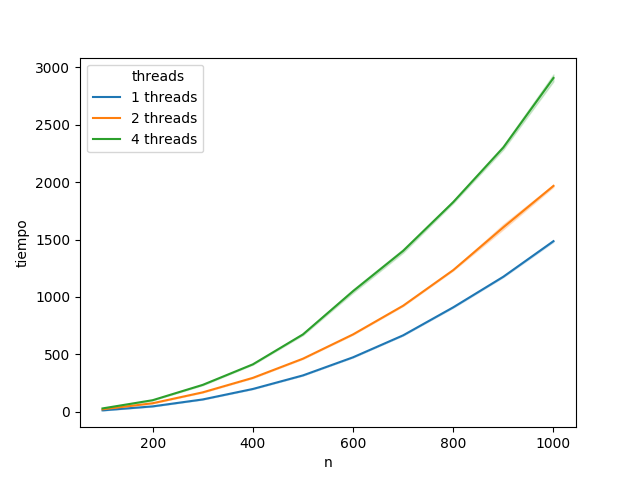
\includegraphics[width=0.5\textwidth]{imagenes/completo-124.png} \\%
\label{fig:completos124}
\end{figure}

La perdida de rendimiento puede deberse a una mala elección o implementación
del algoritmo y las estructuras que le dan soporte. Al incrementar la 
cantidad de \textit{threads} se incrementa el tiempo en el que los mismos se
 encuentran intentando fusionarse. Las fusiones en sí involucran copiar los 
 datos de un thread al otro y reiniciar a uno de ellos. Todas estas son tareas 
 que el algoritmo secuencial no tiene que hacer. Por otro lado, la penalización
  de los cambios de contexto, inexistente en el caso secuencial, es cada vez 
  mayor a medida que crece la cantidad de threads.
% FIXME tirar más hipotesis.

\newpage
\input{4-analisis}
\newpage
\section{Conclusiones y trabajo futuro}

Gracias a los experimentos realizados en el presente trabajo, se pudo llegar a la conclusión de que las ventajas que puede brindar el paradigma \textbf{SIMD} a la hora de implementar programas que realicen operaciones altamente paralelizables, como el procesamiento de imágenes, son verdaderamente significativas. Esto queda reflejado en la gran brecha de rendimiento que se observa entre algunas implementaciones realizadas con dicho paradigma y las que utilizan el lenguaje de programación C.

Esto siempre debe contraponerse a otro hecho que se hizo presente durante el proceso de implementación: realizar un programa en lenguaje ensamblador resulta, por lo general, considerablemente más difícil que hacerlo en un lenguaje de más alto nivel. El código resultante es menos legible, es más sencillo cometer errores y el proceso de \emph{debugging} se vuelve considerablemente más arduo. Por eso es importante analizar de antemano las características del contexto particular de aplicación, para poder decidir si este esfuerzo adicional realmente vale la pena.

Incluso una vez realizada una implementación en ASM, es necesario comparar el rendimiento de ambas versiones con distintos tamaños de imágenes para ver que efectivamente haya una mejora y el grado de la misma -por ejemplo, en nuestras implementaciones Offset para tamaños grandes obtuvo peores resultados que la versión en C con O3-. Otros aspectos a tener en consideración es el tamaño de los binarios involucrados, que puede ser decisivo en determinados escenarios.

También se intentó la realización de una optimización manual dentro del código ensamblador, con distintos resultados. Por ejemplo: expander los ciclos, inlinear llamadas a funciones, analizar instrucciones individuales para encontrar alternativas, tuvieron distintos beneficios en algunos casos y en otros no. Estas optimizaciones son realizadas por el compilador de C al setear alguna opción del flag O, las distintas técnicas de optimización que realizan los mismos pueden servir de inspiración a la hora de intentar mejorar el rendimiento de un programa, pero su justificación siempre tendrá que ser acompañada de métricas que las respalden.

Por último, pudimos hacer una pequeña prueba con la extensión del modelo de SIMD propuesto por la tecnología AVX2 cuyos resultados confirmaron las ventajas de su utilización en la programación vectorial a bajo nivel.

Esperamos que la experiencia nos provea de nuevos recursos a la hora de afrontar problemáticas similares en el futuro.
\end{document}
